\documentclass[../main.tex]{subfiles}
\graphicspath{{\subfix{../IMAGES/}}}

\begin{document}
\localtableofcontents

\subsection{Introduction}
Tous les fluides sont compressibles, les écoulements par contre sont différents : \begin{itemize}
    \item écoulements incompressibles : $\rho$ = constant \begin{itemize}
        \item conservation de la masse\\
        \item conservation de la quantité de mouvement\\
    \end{itemize}
    \item écoulements compressibles : $\rho \neq$ constant \begin{itemize}
        \item conservation de la masse\\
        \item conservation de la quantité de mouvement\\
        \item conservation de l'énergie\\
    \end{itemize}
\end{itemize}

On peut également faire intervenir le nombre de Mach, rapport de la vitesse de l'écoulement u sur la vitesse du son a : \begin{equation}
    M = \frac{u}{a}
\end{equation}

Un écoulement est compressible lorsque $M>0.3$ dans l'air.\\

\subsection{Thermodynamique}
\begin{itemize}
    \item Variable d'état : quantité dépendante de l'état du système\\
    \item Grandeur de parcours : quantité dépendante de l'histoire du système\\
\end{itemize}

\quad \underline{Bivariance d'un système :}\\
Un système est bivariant si son état est entièrement défini par : \begin{itemize}
    \item sa composition chimique\\
    \item sa masse\\
    \item 2 variables d'états indépendantes\\
\end{itemize}

Conditions nécessaires et suffisantes : \begin{itemize}
    \item système monophasé\\
    \item système en équilibre thermique et mécanique\\
\end{itemize}

On définit le \textbf{volume spécifique} : $\nu = \frac{1}{\rho}$ [m$^3$/kg]\\

\begin{equation}
    de_t = de + de_{cin} + de_{pot} = \delta q + \delta w \quad [J/kg]
\end{equation}

Avec : \begin{itemize}
    \item $de_t$ : la variation d'énergie spécifique (massique) totale\\
    \item $de$ : la variation d'énergie interne spécifique\\
    \item $de_{cin} = \frac{1}{2}V^2$\\
    \item $de_{pot} = gh$\\
\end{itemize}

Soit la \textbf{chaleur spécifique} : $c = \frac{\partial q}{dT}$\\
On définit égaiement l'\textbf{enthalpie} : \begin{equation}
    h = e+pv
\end{equation}

Nous pouvons trouver plusieurs relations pour les chaleur spécifiques à température et pression constante : \begin{itemize}
    \item énergie : \begin{itemize}
        \item $c_\nu = (\frac{\partial e}{\partial T})_\nu$\\
        \item $c_p = (\frac{\partial e}{\partial T})_\nu + ((\frac{\partial e}{\partial \nu})_T+p)(\frac{\partial \nu}{\partial T})_p $\\
    \end{itemize}
    \item enthalpie : \begin{itemize}
        \item $c_p = (\frac{\partial h}{\partial T})_p$\\
        \item $c_\nu = (\frac{\partial h}{\partial T})_p + ((\frac{\partial h}{\partial p})_T-\nu)(\frac{\partial p}{\partial T})_\nu$\\
    \end{itemize}
\end{itemize}

\begin{equation}
    \begin{gathered}
        c_p-c_v =  ((\frac{\partial e}{\partial \nu})_T+p)(\frac{\partial \nu}{\partial T})_p = (\nu - (\frac{\partial h}{\partial p})_T)(\frac{\partial p}{\partial T})_\nu \\
        \gamma = \frac{c_p}{c_v} = \frac{(\frac{\partial h}{\partial T})_p}{(\frac{\partial e}{\partial T})_\nu}\\
    \end{gathered}
\end{equation}

Où $\gamma$ est le rapport des chaleurs spécifiques. ($\gamma_{air} = 1.4$)\\

Introduction d'une nouvelle variable d'état s : \textbf{entropie}.\begin{equation}
    ds = \frac{\delta q}{T} + \delta s_i
\end{equation}

$\delta s_i = 0$ si la transformation est réversible, sinon $\delta s_i >0$.\\

\textbf{Relations de GIBBS, valables pour toute transformation, réversible ou irréversible} : \begin{equation}
    Tds = de + pd\nu = dh - \nu dp
\end{equation}

On a également les relations : \begin{itemize}
    \item $(\frac{\partial s}{\partial T})_p = \frac{c_p}{T}$\\
    \item $(\frac{\partial s}{\partial p})_T = \frac{1}{T}[(\frac{\partial h}{\partial p})_T-\nu]$\\
    \item $(\frac{\partial h}{\partial p})_T = \nu - T(\frac{\partial \nu}{\partial T})_p = \frac{1}{\rho} + \frac{T}{\rho^2} (\frac{\partial \rho}{\partial T})_p$\\
\end{itemize}

On obtient alors les relations : \begin{itemize}
    \item $(\frac{\partial e}{\partial \nu})_T + T(\frac{\partial p}{\partial T})_\nu -p$\\
    \item $(\frac{\partial e}{\partial \rho})_T = \frac{1}{\rho^2}(p-T(\frac{\partial p}{\partial T}_\rho))$\\
    \item $\Delta s = \int_1^2 \frac{c_\nu}{T}dT + \int_1^2 (\frac{\partial p}{\partial T})_\nu d\nu = \int_1^2 \frac{c_p}{T}dT - \int_1^2 (\frac{\partial \nu}{\partial T})_p dp$\\
\end{itemize}

Une transformation est isentrope si $ds=0$\\
Elle est adiabate si $\delta q=0$ et elle est réversible si $\delta s_i = 0$\\

\warning La propagation acoustique est largement adiabatique pour $f<<10^9Hz$\\

Dès lors, $p = p(\rho)$.\\
La \textbf{célérité du son} est telle que : \begin{equation}
    a = \sqrt{(\frac{\partial p}{\partial \rho})_s}
\end{equation}

Pour un gaz parfait, on suppose une distance infiniment grande entre les molécules, énergie potentielle nulle et donc sous forme cinétique uniquement.\\

\begin{equation}
    p = \rho r T
\end{equation}
Avec $r = \frac{R}{M}$, $R = 8.314 J/(K mol)$ et $M$ la masse molaire de l'élément.\\

$M_{air} = 29g/mol \rightarrow r_{air} = 287 J/(K kg)$\\

Pour un gaz parfait, l'énergie interne et l'enthalpie ne dépendent que de la température statique.\\

Pour une transformation : \begin{itemize}
    \item avec $c_\nu$ constant : $e = c_\nu T+cst$, $\Delta s = c_\nu \ln(\frac{T_2}{T_1})+r\ln(\frac{\nu_2}{\nu_1})$\\
    \item avec $c_p$ constant : $h = c_p T+cst$, $\Delta s = c_p \ln(\frac{T_2}{T_1})-r\ln(\frac{p_2}{p_1})$\\
\end{itemize}

Relation de Meyer pour un gaz parfait : \begin{equation}
    \begin{gathered}
        c_p-c_\nu = r\\
        1-\frac{c_\nu}{c_p} = \frac{r}{c_p}\\
        c_p = \frac{\gamma r}{\gamma-1}\\
        c_\nu = \frac{r}{\gamma-1}\\
    \end{gathered}
\end{equation}

On a dès lors : $\frac{\Delta s}{r} = \ln(\frac{T_2}{T_1})^\frac{\gamma}{\gamma-1}-\ln(\frac{p_2}{p_1}) = \ln(\frac{T_2}{T_1})^\frac{1}{\gamma-1}+ \ln(\frac{\nu_2}{\nu_1})$\\
Comme la transformation est isentrope : \\
\begin{equation}
    (\frac{p_2}{p_1}) = (\frac{T_2}{T_1})^\frac{\gamma}{\gamma-1} = (\frac{\rho_2}{\rho_1})^\gamma
\end{equation}

Soit :\\
\begin{equation}
    a^2 = (\frac{\partial p}{\partial \rho})_s = \gamma r T
\end{equation}

\warning Où $(\frac{\partial p}{\partial \rho})_s = \gamma (\frac{\partial p}{\partial \rho})_T$ est valide pour tout fluide.\\



La compressibilité isentrope vaut : \begin{equation}
    \alpha_s = \frac{1}{V} (\frac{\partial V}{\partial p})_s = \frac{1}{\nu} (\frac{\partial \nu}{\partial p})_s = -\frac{1}{\rho} (\frac{\partial \rho}{\partial p})_s
\end{equation}

Pour un gaz parfait, on a $\alpha_s p = -\frac{1}{\gamma}$ alors que pour un liquide $\alpha_s p<<1$\\

On définit également le \textbf{module d'élasticité isentrope} : \begin{equation}
    K_s = -\frac{1}{\alpha_s} = \rho (\frac{\partial p}{\partial \rho})_s = \rho a^2
\end{equation}

Le nombre de Mach caractérise la compressibilité d'un écoulement : $M^2 = \frac{\rho u^2 S}{K_s S} \simeq \frac{F_{\text{inertie}}}{F_{\text{élastique}}}$\\

L'écoulement est compressible lorsque les forces d'inertie dominent les forces élastiques responsables de la propagation des ondes de pression.\\

\subsubsection{Chaleurs spécifiques}

L'énergie moléculaire moyenne est égale à : $\varepsilon = \frac{f}{2}kT$, $f$ est le nombre de coordonnées généralisées.\\

L'énergie interne spécifique d'un gaz vaut donc : $e = \frac{f}{2}rT$ et l'enthalpie spécifique $h = \frac{f+2}{2}rT$.\\

Ainsi : \begin{itemize}
    \item $c_\nu = \frac{f}{2}r$\\
    \item $c_p = \frac{f+2}{2}r$\\
\end{itemize}

\begin{equation}
    \gamma = \frac{f+2}{f}
\end{equation}

\begin{table}[hbt!]
    \centering
    \begin{tabular}{c|c|c}
        Type & Nombre degré de liberté & $\gamma$ \\
        \hline
        Monoatomique & 3 & $\frac{5}{3} = 1.67$\\
        Pluriatomique & $f$ grand & $\gamma \rightarrow 1$\\
        Diatomique & 7 & $\frac{9}{7} = 1.286$\\
    \end{tabular}
\end{table}

\warning Pour un gaz quelconque : $1<\gamma \leq1.67$

Les degrés de liberté ne sont activés qu'à certaines températures d'activation ! A des températures ambiantes, les gaz diatomiques n'ont que 5 degrés de liberté : $\gamma = \frac{7}{5} = 1.4$\\

\subsection{Équations fondamentales}

\subsubsection{Conservation de la masse}

\begin{equation}
    \frac{\partial \rho}{\partial t} + \nabla \cdot (\rho \Vec{u}) = 0
\end{equation}

On peut également l'exprimer selon la dérivée matérielle/totale : $\frac{DF}{Dt} = \frac{\partial F}{\partial t} + \Vec{u}\cdot \nabla F$\\

Soit : $\frac{D \rho}{Dt} + \rho \nabla \cdot \Vec{u} = 0$\\

On a dès lors le tenseur de contraintes : $\nabla \cdot \underline{\underline{\sigma}} = -\nabla p + \nabla \cdot \underline{\underline{\tau}}$\\

Pour les gaz parfaits : $\underline{\underline{\sigma}} = -p \underline{\underline{I}}$\\

On obtient dès lors la formulation d'Euler de la conservation de quantité de mouvement : \begin{equation}
    \rho \frac{D \Vec{u}}{Dt} = -\nabla p + \rho \Vec{f}
\end{equation}

Pour des fluides parfaits, on a la formulation de Lamb : $(\frac{\partial \Vec{u}}{\partial t} - \Vec{u} \times \Vec{\omega}) = -\frac{1}{\rho} \nabla p - \nabla \frac{u^2}{2} + \Vec{f}$\\

Voire celle de Crocco : $(\frac{\partial \Vec{u}}{\partial t} - \Vec{u} \times \Vec{\omega}) = -\nabla h_0 + T\nabla s + \Vec{f}$, $h_0 = h + \frac{u^2}{2}$\\

Selon cette formulation, si le fluide est stationnaire, à force volumique nulle, isentropique et irrotationnel (soit l'écoulement est irrotationnel soit on se trouve le long d'une ligne de courant), on obtient : $\nabla h_0 = 0$\\

Pour les gaz parfaits, on a : \begin{equation}
    \begin{gathered}
        \rho \frac{D(e_0)}{Dt} = \frac{\partial(\rho e_0)}{\partial t} + \nabla \cdot (\rho e_0 \Vec{u}) = -\nabla \cdot (\rho \Vec{u}) + \rho \Vec{f} \cdot \Vec{u} - \nabla \cdot \Vec{q} + r\\
        \rho \frac{D(h_0)}{Dt} = \frac{\partial(\rho h_0)}{\partial t} + \nabla \cdot (\rho h_0 \Vec{u}) = \frac{\partial p}{\partial t} + \rho \Vec{f} \cdot \Vec{u} - \nabla \cdot \Vec{q} + r\\
    \end{gathered}
\end{equation}

De plus, on a la fonction de dissipation visqueuse : $\underline{\underline{\tau}}:\nabla \Vec{u} \geq 0$\\

Pour un fluide sans viscosité et adiabatique, on a $\frac{Ds}{Dt} = 0$\\

\subsection{Écoulement isentrope permanents}
\warning Une onde se propage toujours à la même vitesse dans toutes les directions selon un référentiel dans le fluide !\\

Lorsque l'émetteur d'onde se déplace supersoniquement, on forme un cône de Mach avec pour demi-angle au sommet : \begin{equation}
    \sin \mu = \frac{1}{M}
\end{equation}

Une onde de Mach/ligne de Mach/cône de Mach est \textbf{une onde de pression d'intensité infinitésimale} par rapport à la pression ambiante ($\Delta p << p_{ambiant}$, $\frac{\Delta p}{p} \simeq 1\%$)\\

Si on considère un écoulement isentrope permanent, on a : \begin{itemize}
    \item fluide dénué de viscosité\\
    \item pas de forces volumiques $\Vec{f} = 0$ ni de rayonnement $r=0$ ni de transfert de chaleur $\nabla \cdot \Vec{q}=0$\\
\end{itemize}

Si on considère le cas permanent de la conservation de la quantité de mouvement : $\rho \frac{D\Vec{v}}{Dt} = -\nabla p \Rightarrow \Vec{v} \cdot \nabla \Vec{v} = -\frac{1}{\rho} \nabla p$\\
Le long d'une ligne de courant, on a donc : \begin{equation}
    \frac{v^2}{2} + \int \frac{dp}{\rho} = cst
\end{equation}

De la même manière, dans le cas permanent pour la conservation d'énergie : $\frac{D h_0}{Dt} = \frac{1}{\rho} \frac{\partial p}{\partial t} \Rightarrow \Vec{v} \cdot \nabla h_0 = 0$\\
Le long d'une ligne de courant on a donc : \begin{equation}
    h_0 = h + \frac{v^2}{2} = cst
\end{equation}

\subsubsection{Grandeurs totales}
\begin{itemize}
    \item \textbf{Un point d'arrêt} d'un écoulement permanent est un point où la vitesse est nulle\\
    \item Une grandeur totale est une grandeur définie en un point d'arrêt d'un écoulement permanent\\
\end{itemize}

On les note $h_0$, $T_0$, $\rho_0$, $p_0$, $s_0$ et on a la propriété $v = v_0 = 0$\\

La température totale $T_0$ est constante pour un écoulement isentrope permanent.\\

Pour un gaz parfait, on a $c_pT + \frac{v^2}{2} = c_p T_0$.\\

\begin{itemize}
    \item \textbf{Un point sonique} d'un écoulement est un point où la vitesse est égale à la célérité du son\\
    \item Une grandeur sonique est une grandeur définie en un point aux conditions soniques.\\
\end{itemize}

On les note $h_*$, $T_*$, $\rho_*$, $p_*$, $s_*$ et on a la propriété $v = v_* = a_*$\\


On peut maintenant réécrire l'équation de conservation d'énergie : \begin{equation}
\begin{gathered}
    \frac{T_0}{T} = 1+\frac{\gamma-1}{2} (\frac{v}{a})^2 = 1+ \frac{\gamma-1}{2} M^2\\
    \frac{p_0}{p} = (1+\frac{\gamma-1}{2}M^2)^{\frac{\gamma}{\gamma-1}}\\
    \frac{\rho_0}{\rho} = (1+\frac{\gamma-1}{2}M^2)^{\frac{1}{\gamma-1}}\\
    \end{gathered}
\end{equation}

Le long d'une ligne de courant, on a donc : \begin{equation}\begin{gathered}
    \frac{a^2}{\gamma-1} + \frac{v^2}{2} = \frac{a_0^2}{\gamma-1} = \frac{\gamma+1}{2(\gamma-1)}a_*^2 = cst\\
    \frac{a^2}{a_0^2} = (1+\frac{\gamma-1}{2}M^2)^{-1}\\
    \end{gathered}
\end{equation}

Dès lors, $\frac{dv}{v} = \frac{1}{1+\frac{\gamma-1}{2}M^2} \frac{dM}{M}$\\

\begin{itemize}
    \item Si $v> a_* \Leftrightarrow a_*> a \Rightarrow v>a \Rightarrow M>1$ écoulement supersonique\\
    \item Si $v< a_* \Leftrightarrow a_*< a \Rightarrow v<a \Rightarrow M<1$ écoulement subsonique\\
\end{itemize}

On peut également exprimer le nombre de Mach associé aux grandeurs soniques : $M_* = \frac{v}{a_*}$\\

\begin{equation}
    \begin{gathered}
        M_*^2 = \frac{(\gamma+1) M^2}{2+(\gamma-1)M^2}\\
        M^2 = \frac{2}{\frac{\gamma+1}{M_*^2} - (\gamma-1)}\\
    \end{gathered}
\end{equation}

\warning Le nombre de Mach représente une mesure des variations relatives de masse volumique, soit l'erreur qu'on commet en considérant une masse volumique constante.\\

\subsection{Écoulement quasi-mono-dimensionnel isentropiques permanents}
En supposant un écoulement mono-dimensionnel $u(x)$ et permanent, on obtient pour la \textbf{conservation de la masse} $\frac{d}{dx}(\rho u A)=0$\\

On a dès lors \begin{equation}
\frac{u}{\sqrt{2 c_p T_0}} = \sqrt{\frac{\gamma-1}{2}} \frac{M}{\sqrt{1+\frac{\gamma-1}{2}M^2}}
\end{equation}
\warning Lorsque $M\rightarrow \infty$, on a $\frac{u}{\sqrt{2 c_pT_0}} \rightarrow 1$\\

\begin{figure}[hbt!]
    \centering
    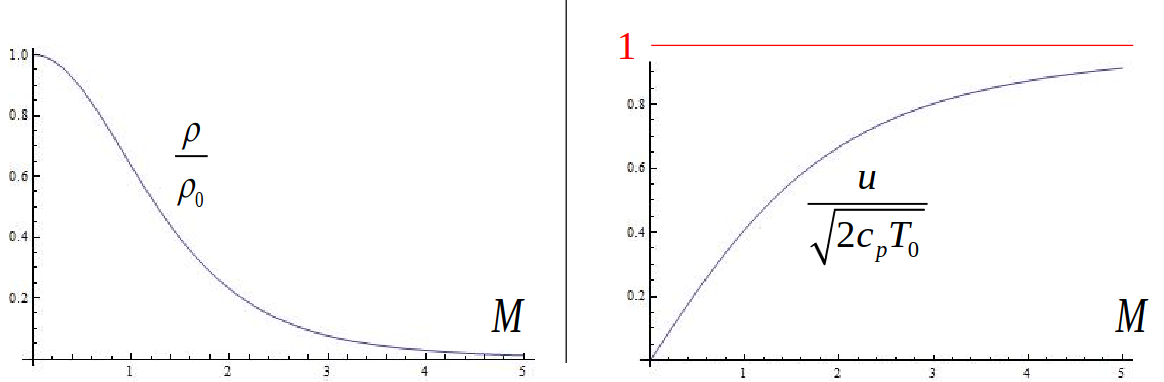
\includegraphics[width=.6\textwidth]{IMAGES/machineelec/debit_surf.png}
\end{figure}

De plus, pour un débit par unité de surface : \begin{equation}
    \frac{\rho u}{\rho_0 \sqrt{2c_p T_0}} = \sqrt{\frac{\gamma-1}{2}} \frac{M}{(1+\frac{\gamma-1}{2}M^2)^{\frac{\gamma+1}{2(\gamma-1)}}}
\end{equation}

\begin{figure}[hbt!]
    \centering
    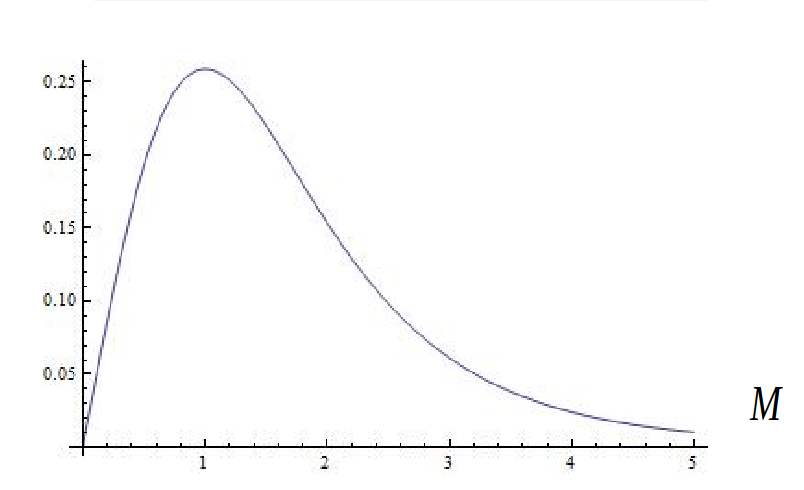
\includegraphics[width = .5\textwidth]{IMAGES/machineelec/debit_usurf.png}
\end{figure}

Une tuyère convergente-divergente est nécessaire pour passer d'un régime subsonique à un régime supersonique.\\

\begin{figure}[hbt!]
    \centering
    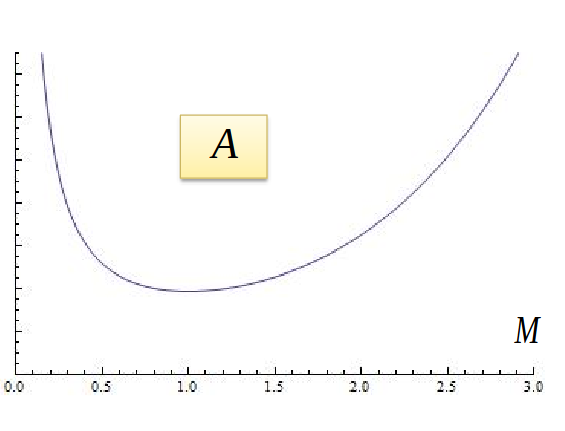
\includegraphics[width = .5\textwidth]{IMAGES/machineelec/aire.png}
\end{figure}

On considère maintenant un fluide sans viscosité ni forces volumiques $\sigma = -pI$, $\Vec{f} = 0$\\

On obtient par la quantité de mouvement : $\rho u \frac{du}{dx} = -\frac{dp}{dx}$\\

Enfin : \begin{equation}
    \frac{d\rho}{\rho} + \frac{du}{u} + \frac{dA}{A} = 0
\end{equation}
Comme l'écoulement est \textbf{isentrope}, on a $\frac{dp}{\rho} = -udu$ ainsi que $\frac{d\rho}{\rho} = -M^2 \frac{du}{u}$ soit : \begin{equation}
    \frac{dA}{A} = (M^2-1)\frac{du}{u}
\end{equation}

On a dès lors : \begin{table}[hbt!]
    \centering
    \begin{tabular}{ccccc}
    \hline
        dA/A & - & - & + & + \\
        M & <1 & >1 & <1 & >1\\
        \hline
        du/u & + & - & - & +\\
        dM/M & + & - & - & +\\
        \hline
        dp/p & - & +& + & -\\
        d$\rho$/$\rho$ & - & + & + & -\\
        dT/T & -& + & + &-\\
        da/a & - & + & + &-\\
    \end{tabular}
\end{table}

Comme : $\lim_{M\rightarrow 1, \frac{dA}{dx}\rightarrow 0} (\frac{dM}{dx})^2 = \frac{(1+\gamma)}{4A} \frac{d^2A}{dx^2}\geq 0$, on a $\frac{d^2A}{dx^2} \geq 0$\\
\textbf{Le passage du régime subsonique au régime supersonique s'effectue au col de la tuyère (minimum)}\\

Le nombre de Mach n'est fonction que de $A/A_*$ : \begin{equation}
    \frac{A}{A_*} = \frac{1}{M} [\frac{2}{\gamma+1} (1+\frac{\gamma-1}{2}M^2)]^{\frac{\gamma+1}{2(\gamma-1)}}
\end{equation}

On peut également l'exprimer selon la pression : $\frac{A_*}{A} = \sqrt{\frac{2}{\gamma-1} (\frac{2}{\gamma+1})^{-\frac{\gamma+1}{\gamma-1}}} (\frac{p}{p_0})^{\frac{1}{\gamma}} \sqrt{1-(\frac{p}{p_0})^{\frac{\gamma-1}{\gamma}}}$\\

Soit le débit massique : \begin{equation}
    \begin{gathered}
        \dot{m} = \gamma M (1+\frac{\gamma-1}{2}M^2)^{-\frac{\gamma+1}{2(\gamma-1)}}\frac{p_0}{a_0} A\\
        \frac{\dot{m}}{\rho_0 a_0 A_*} = (1+\frac{\gamma-1}{2})^{-\frac{\gamma+1}{2(\gamma-1)}}\\
    \end{gathered}
\end{equation}

\begin{itemize}
    \item Écoulement subsonique : $p_{sortie} = p_{ambiante}$\\
    \item Écoulement supersonique : \begin{itemize}
        \item sur-détendu : $p_{\text{sortie}} < p_{\text{arrière}}$\\
        \item point de fonctionnement : $p_{\text{sortie}} = p_{\text{arrière}}$\\
        \item sous-détendu : $p_{\text{sortie}} > p_{\text{arrière}}$\\
    \end{itemize}
\end{itemize}

\warning Le long d'un écoulement, le débit est constant.\\

\begin{equation}
    \frac{\dot{m} \sqrt{rT_0}}{p_0 A} = \sqrt{\frac{2\gamma}{\gamma-1}} (\frac{p}{p_0})^{\frac{1}{\gamma}} \sqrt{1-(\frac{p}{p_0})^{\frac{\gamma-1}{\gamma}}} = \sqrt{\gamma} M (1+\frac{\gamma-1}{2}M^2)^{-\frac{\gamma+1}{2(\gamma-1)}}
\end{equation}

Dans une tuyère convergente, au maximum au col on a M=1\\

\subsection{Ondes de chocs/détente}
\subsubsection{Ondes de chocs}
Une onde de choc est une zone de l'espace où les grandeurs physiques subissent de très fortes variations sur une distance très faible. On les idéalise comme des surfaces de discontinuités. \\
\warning Les grandeurs physiques sont discontinues à travers une onde de choc.\\
Deux types : \begin{itemize}
    \item Chocs droits (normal à l'écoulement), M diminue, p T $\rho$ augmentent\\
    \item Chocs obliques, M diminue, T p et $\rho$ augmentent\\
\end{itemize}

\subsubsection{Ondes de détente}
Une onde de détente est une zone de l'espace où la pression décroît de manière continue. On a accélération du fluide, p T et $\rho$ diminuent.\\

En appliquant la conservation de quantité de mouvement sur la surface de contrôle autour de l'onde au repos, on a : \begin{equation}
    dp = \rho a du
\end{equation}

Lorsque deux ondes se suivent et avancent à une vitesse supersonique dans leur milieu, on a plusieurs effets : \begin{itemize}
    \item la première onde se propage à la vitesse du son dans le fluide 1\\
    \item la deuxième onde va surfer sur le fluide 2 se déplaçant à la vitesse du, va se propager à la vitesse du son du fluide 2 et va se propager dans le référentiel du fluide 1 à une vitesse $a_2 + du >a_1$\\
\end{itemize}

Dès lors, lorsque deux ondes de compression se suivent, elles vont se rattraper et former une onde de compression de grande amplitude; une onde de choc.\\
A l'inverse, deux ondes de détente ne se rattrapent jamais.\\

On a ($u_w$ : vitesse de l'onde, $u$ : vitesse du fluide, $a$ : vitesse du son) \begin{equation}
    \frac{du_w}{dp} = \frac{du}{dp} + \frac{da}{dp}
\end{equation}

Soit $\Gamma = \frac{\gamma+1}{2}$ pour un gaz parfait. On a \begin{equation}\frac{du_w}{dp} = \frac{\Gamma}{\rho a}\end{equation}

La variation de la vitesse de l'onde avec la pression dépend du signe de $\Gamma$, pour un gaz parfait $\Gamma > 1$n pour la plupart des fluides $\Gamma > 0$\\
Pour des fluides normaux, on obtient des chocs de compression.\\

Or $\Gamma = \frac{a^4}{2\nu^3} (\frac{\partial^2 \nu}{\partial p^2})_s$\\
Pour des fluides proches du point critique, on peut avoir des chocs de détente.\\

\subsubsection{Ondes de choc droites}
La vitesse de l'écoulement est normale à l'onde. On se place toujours dans un référentiel fixe par rapport au choc.\\

Soit un volume de contrôle tel que, il possède un volume infinitésimal, des surfaces parallèles d'aire égales, des surfaces latérales d'aires négligeables.\\

On a par les lois suivantes : \begin{itemize}
    \item Conservation de la masse : $[\rho w_n] = 0$\\
    \item Conservation de la quantité de mouvement : $[\rho w_n^2 + p] = 0$\\
    \item Conservation de l'énergie : $[h + \frac{w_n^2}{2}] = 0$\\
    \item 2ème principe de Thermodynamique : $[s]>0$\\
\end{itemize}

On définit le \textbf{Nombre de Mach du choc} \begin{equation}
    M_{n,1} = \frac{w_{n,1}}{a_1}
\end{equation}

\warning La température totale ne change pas à travers un choc droit.\\

On a pour des gaz parfaits: \begin{itemize}
    \item $\frac{T_2}{T_1} = \frac{h_2}{h_1} = \frac{1+ \frac{\gamma-1}{2} M_{n,1}^2}{1+\frac{\gamma-1}{2}M_{n,2}^2}$\\
    \item $\frac{\rho_2}{\rho_1} = \frac{(1+\gamma M_{n,1}^2)T_1}{(1+\gamma M_{n,2}^2)T_2}$\\
    \item $M_{n,2}^2 = \frac{(1+\frac{\gamma-1}{2} M_{n,1}^2)}{\gamma M_{n,1}^2 - \frac{\gamma-1}{2}}$\\
\end{itemize}

En introduisant les relations isentropes, on a : (valable de chaque côté du choc) \begin{itemize}
    \item $\frac{p_{0,2}}{p_{0,1}} = \frac{p_2}{p_1} (\frac{1+ \frac{\gamma-1}{2} M_{n,2}^2}{1+ \frac{\gamma-1}{2} M_{n,1}^2})^{\frac{\gamma}{\gamma-1}} = e^{-\frac{s_2-s_1}{r}}$\\
    \item $s_2-s_1 = c_v \ln([1+\frac{2\gamma}{\gamma+1}(M_{n,1}^2-1)][1-\frac{2}{\gamma+1} \frac{M_{n,1}^2-1}{M_{n,1}^2}]^\gamma )$\\
    \item $\frac{p_{0,2}}{p_{0,1}} = e^{-\frac{s_2-s_1}{r}}$\\
\end{itemize}

\warning Les chocs droits n'apparaissent que pour $M_{n,1} \geq 1$.\\

On obtient également la relation de Rankine-Hugoniot : $\frac{p_2}{p_1} = \frac{1+\frac{\rho_1}{\rho_2} - \frac{2\gamma}{\gamma-1}}{1-\frac{\gamma+1}{\gamma-1} \frac{\rho_1}{\rho_2}}$ \\
\warning On ne considère ici pas les relations isentropes !\\

La pression croît à travers un choc. l'écoulement est toujours \textbf{supersonique à l'amont et subsonique à l'aval d'un choc droit}.\\

\subsubsection{Ondes de choc droites dans un fluide quelconque}
On a : $h_2-h_1 = \frac{p_2-p_1}{2} (\frac{1}{\rho_1} + \frac{1}{\rho_2}) = \frac{\nu_1 + \nu_2}{2} (p_2-p_1)$\\

Les équations de conservation de la masse, quantité de mouvement et d'énergie sont les mêmes : $[\rho w_n] = [\rho w_n^2 + p] = [h + \frac{w_n^2}{2}] = 0$\\

On a ainsi les relations : \begin{itemize}
    \item $w_{n,1}w_{n,2} = \frac{[p]}{[\rho]}$\\
    \item $j^2 = -\frac{[p]}{[\nu]}$\\
    \item $\Pi = -M_{n,1} \frac{[w_n]}{a_1} = -M_{n,1}^2 \frac{[\nu]}{\nu_1} = \frac{[p]}{\rho_1 a_1^2}$, mesure de l'intensité du choc\\
    \item $[w_n]^2 = -[p][\nu]$\\
\end{itemize}

Choc faible $\Pi <<1$, choc fort $\Pi >> 1$\\

Par la relation de Rankine-Hugoniot, on a : $\frac{[s]}{a_1^2/T_1} = \frac{1}{6} \Gamma_1 \Pi^3$\\

\subsubsection{Applications}
Si l'on met deux tuyères en bout de l'autre (la première avec un col plus serré que la deuxième), on a $a_{*,1} = a_{*,2} = a_*$\\
De plus, $w_{n,2} - w_{n,1} = \frac{p_1}{\rho_1 w_{n,1}} - \frac{p_2}{\rho_2 w_{n,2}}$, $\frac{p}{\rho w_n} = \frac{\gamma+1}{2\gamma} \frac{a_*^2}{w_n} - \frac{\gamma-1}{2\gamma} w_n$\\

La relation de Prandtl nous donne : $w_{n,1} w_{n,2} = a_*^2 = \frac{2}{\gamma+1} a_0^2$\\

On a dès lors le résultat : \begin{equation}
    p_{0,1} A_{*,1} = p_{0,2} A_{*,2}
\end{equation}
Lors d'un choc entre les deux tuyères. \\

\quad \underline{Entrée d'air supersonique :}\\
Au démarrage, le nombre de mach avant la turbine est inférieur à 1. Ensuite, lorsque le nombre de Mach en aval dépasse 1 $M_0>1$ on a formation d'une onde de choc droite devant l'entrée d'air supersonique. Si l'avion accélère au delà de son nombre de Mach de vol, l'onde de choc se déplace dans la turbine. Le choc est alors avalé vers une position stable. La turbine peut alors ralentir pour mettre le choc légèrement plus loin que le col.\\

\quad \underline{Tube Pitot supersonique :}\\
On a une onde de choc devant le tube.\\

La formule de Rayleigh nous donne : \begin{equation}
    \frac{p_{0,2}}{p_1} = \frac{(\frac{\gamma+1}{2} M_1^2)^{\frac{\gamma}{\gamma-1}}}{(\frac{2\gamma}{\gamma+1} M_1^2 - \frac{\gamma-1}{\gamma+1})^{\frac{1}{\gamma-1}}}
\end{equation}

Pour mesurer la pression statique $p_1$, deux moyens : \begin{itemize}
    \item sur la paroi en amont du Pitot\\
    \item à une distance de 10 diamètres en aval sur le tube\\
\end{itemize}

\subsection{Écoulement de Prandtl-Meyer}
Dans le cas d'un changement progressif de l'angle de la paroi, il y a apparition d'un faisceau continu d'ondes avec une pression totale constante et une entropie constante.\\
Un choc de détente ne peux pas exister, uniquement une onde de détente dans laquelle, la pression totale et entropie restent constant.\\
Géométriquement, on a $ \frac{w_{n,2} - w_{n,1}}{w_t} = - \frac{\tan \delta}{ \cos^2 \theta (1+\tan\theta \tan \delta}$\\
$\Pi = \frac{[p]}{\rho_1 a_1^2} = -M_{n,1} \frac{[w_n]}{a_1} \Rightarrow \frac{\Pi}{M_1^2} = \frac{\tan \delta}{ \cot \theta + \tan \delta}$\\

Comme le choc est infiniment faible (proche d'une onde de Mach), on suppose $\theta \rightarrow \mu$, $\delta \rightarrow d\delta$, $\cot \theta \rightarrow \cot \mu = \sqrt{M_1^2-1}$\\

\begin{equation} \begin{gathered}
    \frac{\Pi_{faible}}{M_1^2} = \frac{d\delta}{\sqrt{M_1^2-1}}\\
    \frac{T_1[s]_{faible}}{a_1^2} = \frac{1}{6} \Gamma_1 \frac{M_1^6}{(M_1^2-1)^{3/2}} (d\delta)^3\\
    \end{gathered}
\end{equation}

\warning L'écoulement à travers un faisceau continu de chocs infiniment faibles est isentropique. Le saut en pression est fini et on peut avoir une détente ou une compression.\\

\begin{itemize}
    \item $d\delta >0$ : compression isentrope\\
    \item $d\delta < 0$ : détente isentrope\\
\end{itemize}

\begin{equation}
    d\delta = -\sqrt{M_1^2-1} \frac{dw}{w}
\end{equation}

On peut dès maintenant avoir la relation de Prandtl-Meyer : \begin{equation} \begin{gathered}
    d\delta = -\frac{\sqrt{M^2-1}}{1+\frac{\gamma-1}{2}M^2} \frac{dM}{M}\\
    \nu(M) = \sqrt{\frac{\gamma+1}{\gamma-1}} \arctan \sqrt{\frac{\gamma-1}{\gamma+1}(M^2-1)} - \arctan \sqrt{M^2-1}\\
    \nu_2(M_2) = \nu_1(M_1) - \delta\\
    \end{gathered}
\end{equation}

La fonction de Prandtl-Meyer $\nu$ représente l'angle dont doit s'ouvrir une rampe afin de détendre l'écoulement de M=1 à M.\\

Soit le coefficient de portance : $c_L = \frac{F_L}{1/2 \rho_\infty u_\infty^2 c} = \frac{F_L}{1/2  \gamma p_\infty M_\infty^2 c}$\\
Ainsi que le coefficient de traînée : $c_D = \frac{F_D}{1/2 \rho_\infty u_\infty^2 c}$\\





\end{document}